Let $\module{F}$ be a quasi-coherent module on $\overcat{C}{a}$.
We have to show that $\sections{a}{F} \tensor_{\sections{a}{O}} \sections{b}{O} \xrightarrow{f} \sections{b}{F}$ is an isomorphism, 
where $k$ is the adjunct of $\module{F}(f)$ with respect to the adjunction between restricting scalars and extending scalars along the map 
$\sections{a}{O} \rightarrow \sections{b}{O}$. More concretely, 

\[k: x \tensor m \mapsto \module{F}(f)(x)m.\]

Since $a$ is caffine, $\module{F}= \Tildefunctor{\globalsections{F}}$.
Since $\Tildefunctor = \sheafify{\blank} \circ \Kappa{\blank}$, we know that $\module{F}$ is the sheafification of $c \rightarrow \sections{a}{F} \tensor_{\sections{a}{O}} \sections{c}{O}$.
Set $M = \sections{a}{F}$.

Define $k´: \sections{a}{\Kappa{M}} \tensor_{\sections{a}{O}} \sections{b}{O} \rightarrow \sections{b}{\Kappa{B}}$
By $k':x \tensor m \mapsto \kappa{F}(f)(x) m$.
If you unfold the constructions, it follows that $k'(x\tensor m) = x\tensor m \in \sections{b}{\Kappa{B}} = M \tensor \sections{b}{O}$ is actually the identity.

A) The component at a caffine object of the unversal sheafification morphism $i$ is an isomorphism
As is stated in lemma .. , we have $\globalsections{i} = \counit{\Tildefunctor{\blank}}$. 

Note that the sheafification morphism $i: \Kappa{M} \rightarrow \Tildefunctor{M}$ is the adjunct of the identity $\Tildefunctor{M} \rightarrow \Tildefunctor{M}$ along the sheafification adjunction. So taking the adjunct of $i$ along the $\adjunction{\Kappa}{\globalsection{\blank}}$ yields the adjunct of the identity along the $\mainadjunction$, because $\Tildefunctor = \Kappa \circ \globalsections{\blank}$. which is the counit.
Note that $\globalsections$ is full,

at $\terminal$ has as adjunct the co-unit of $\mainadjunction$, by moving $\Kappa$ to the right to get $\counit: M \rightarrow \globalsections{\Tildefuntor{M}}$. 
Since the global sections on presheaves are an equivalence of categories it reflects isos. So $i$ is an iso for any caffine object.



B) Adjunction bijection respects composition with isos
C) Hence $k$ is also an iso.



Note that restricting and sheafification commute.%TODO: explain
We can first restrict our presheaf to $\cat{C}/b$ and then sheafify. 
The global sections component of the universal sheafification morphism will be 
\[M \tensor \sections{b}{O} \rightarrow \sections{b}{F},\]
\[m \tensor r \mapsto mr\]

because the triangle 

\begin{center}
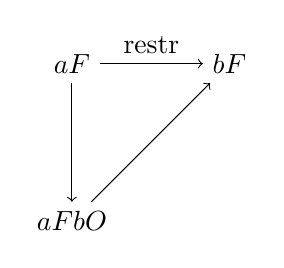
\begin{tikzpicture}[node distance=2cm, auto]
  \node (C) {$\sections{a}{F}$};
  \node (B) [right of =C] {$\sections{b}{F}$};
  \node (D) [below of= C]{$\sections{a}{F}\tensor \sections{b}{O}$};
  \draw[->] (C) to node {$\mbox{restr}$} (B);
  \draw[->] (D) to node [swap] {}  (B);
  \draw[->] (C) to node [swap] {} (D);
\end{tikzpicture}
\end{center}

must commute by naturality. This is exactly the component of the unit $\eta$ of the $\mainadjunction$ on $\site{C}{T}{O}/b$ for $\sections{a}{F} \tensor \sections{b}{O}$.
Since $b$ is caffine, this is an isomorphism by assumption.